\documentclass[a4paper]{article}

% --- Packages ---

\usepackage{a4wide}
\usepackage[utf8]{inputenc}
\usepackage{amsmath}
\usepackage{mathtools}
\usepackage{amssymb}
\usepackage[english]{babel}
\usepackage{mdframed}
\usepackage{systeme,}
\usepackage{lipsum}
\usepackage{relsize}
\usepackage{caption}
\usepackage{tikz}
\usepackage{tikz-3dplot}
\usetikzlibrary{shapes.geometric}
\usepackage{pgfplots}
\usepackage{pgfplotstable}
\pgfplotsset{compat=newest}%1.7}
\usepackage{harpoon}%
\usepackage{graphicx}
\usepackage{wrapfig}
\usepackage{subcaption}
\usepackage{authblk}
\usepackage{float}
\usepackage{listings}
\usepackage{xcolor}
\usepackage{chngcntr}
\usepackage{amsthm}
\usepackage{comment}
\usepackage{commath}
\usepackage{hyperref}%Might remove, adds link to each reference
\usepackage{url}
\usepackage{calligra}
\usepackage{pgf}

% --- Bibtex ---

%\usepackage[backend = biblar,]{bibtex}

%\addbibliografy(ref.bib)

% --- Commands --- 

\newcommand{\w}{\omega}
\newcommand{\trace}{\text{Tr}}
\newcommand{\grad}{\mathbf{\nabla}}
%\newcommand{\crr}{\mathfrak{r}}
\newcommand{\laplace}{\nabla^2}
\newcommand{\newparagraph}{\vspace{.5cm}\noindent}

% --- Math character commands ---

\newcommand{\curl}[1]{\mathbf{\nabla}\times \mathbf{#1}}
\newcommand{\dive}[1]{\mathbf{\nabla}\cdot \mathbf{#1}}
\newcommand{\res}[2]{\text{Res}(#1,#2)}
\newcommand{\fpartial}[2]{\frac{\partial #1}{\partial #2}}
\newcommand{\rot}[3]{\begin{vmatrix}\hat{x}&\hat{y}&\hat{z}\\\partial_x&\partial_y&\partial_z\\#1&#2&#3 \end{vmatrix}}
\newcommand{\average}[1]{\langle #1 \rangle}
\newcommand{\ket}[1]{|#1\rangle}
\newcommand{\bra}[1]{\langle #1|}


%  --- Special character commands ---

\DeclareMathAlphabet{\mathcalligra}{T1}{calligra}{m}{n}
\DeclareFontShape{T1}{calligra}{m}{n}{<->s*[2.2]callig15}{}
\newcommand{\crr}{\mathcalligra{r}\,}
\newcommand{\boldscriptr}{\pmb{\mathcalligra{r}}\,}


\title{Handin 6}
\author{Author : Andreas Evensen}
\date{Date: \today}

% --- Code ---

\definecolor{codegreen}{rgb}{0,0.6,0}
\definecolor{codegray}{rgb}{0.5,0.5,0.5}
\definecolor{codepurple}{rgb}{0.58,0,0.82}
\definecolor{backcolour}{rgb}{0.95,0.95,0.92}

\lstdefinestyle{mystyle}{
    backgroundcolor=\color{backcolour},   
    commentstyle=\color{codegreen},
    keywordstyle=\color{magenta},
    numberstyle=\tiny\color{codegray},
    stringstyle=\color{codepurple},
    basicstyle=\ttfamily\footnotesize,
    breakatwhitespace=false,         
    breaklines=true,                 
    captionpos=b,                    
    keepspaces=true,                 
    numbers=left,                    
    numbersep=5pt,                  
    showspaces=false,                
    showstringspaces=false,
    showtabs=false,                  
    tabsize=2
}

\lstset{style=mystyle}

\begin{document}

\maketitle

\noindent
Consider the free energy density:
\begin{align*}
    \mathcal{L} &= \frac{1}{2}a\eta^2 + \frac{1}{4}b\eta^4 + \frac{1}{6}c\eta^6 - h\eta,
\end{align*}where $ c> 0 $, $a$ and $b$ are both linearly proportional to the pressure $p$ and temperature $T$ near the critical point, $(T_c, p_c)$.
\begin{align*}
    a &= a_1t + a_2p,\quad b = b_1t + b_2p.
\end{align*}Here, $t$ and $p$ are the reduced temperature and pressure, respectively.
As $T$ and $p$ are varied both $a$ and $b$ can be made to vanish or change sign.
Such a system exhibits a tricritical point. An example of this is $He^3$ and $He^4$.
In this question we will calculate the phase diagram in the $a-b$ plane for $h = 0$, using Landau theory.

\section*{a)}
Consider the case $a<0$. Find the extrema for the Landau free energy, and study their stability. Hence, show:
\begin{align*}
    \average{\eta}^2=\eta_s^2 = \frac{-b + \sqrt{b^2 - 4ac}}{2c}.
\end{align*}

\newparagraph
\textbf{Answer: } Since $h = 0$, we're left with the following Landau free energy density (LFD):
\begin{align}
    \mathcal{L} &= \frac{1}{2}a\eta^2 + \frac{1}{4}b\eta^4 + \frac{1}{6}c\eta^6. \label{eq: LFD}
\end{align}Differentiating \eqref{eq: LFD} with respect to $\eta$ gives us the following equation:
\begin{align*}
    \fpartial{\mathcal{L}}{\eta} &= a\eta + b\eta^3 + c\eta^5 = \eta(a + b\eta^2 + c\eta^4).
\end{align*}The solution to $\fpartial{\mathcal{L}}{\eta} = 0$ is $\eta = 0$, and the solutions to the quadratic equation $a + b\eta^2 + c\eta^4 = 0$ are given by:
\begin{align*}
    \eta^2 &= \frac{-b \pm \sqrt{b^2 - 4ac}}{2c} = \eta_s^2.
\end{align*}To study the stability of the extrema, we need to consider the second derivative of the LFD:
\begin{align*}
    \fpartial{^2\mathcal{L}}{\eta^2} &= a + 3b\eta^2 + 5c\eta^4.
\end{align*}
If $a < 0$, and $\eta = 0$, then $\fpartial{^2\mathcal{L}}{\eta^2} = a < 0$, so $\eta = 0$ is a maximum, i.e. unstable.
The two solutions $\eta_s^2$ are minimums by the same argument.


\section*{b)}
Now consider $a>0$, $b>0$. How does $\eta_s$ behave in this region?

\newparagraph
\textbf{Answer: }If $\eta = 0$, then $\fpartial{^2\mathcal{L}}{\eta^2} = a > 0$, so $\eta = 0$ is a minimum, i.e. stable.
The 'stable' solutions $\eta_s^2$ then can only be saddle points or not valid solutions. We can see this by considering the second derivative of the LFD. If saddle points exist, the second derivative should be zero, otherwise it's a false solution.
\begin{align*}
    \fpartial{^2\mathcal{L}}{\eta^2} &= a + 3b\eta^2 + 5c\eta^4\\
    &= a + 3b\eta_s^2 + 5c\eta_s^4\\
    &= a + 3b\frac{-b \pm \sqrt{b^2 - 4ac}}{2c} + 5c\frac{\left(-b \pm \sqrt{b^2 - 4ac}\right)^2}{4c^2}\neq 0.
\end{align*}Hence, the only solution is $\eta = 0$.
\section*{c)}
Lastly, consider $a>0$, $b<0$. What happens here?

\newparagraph
\textbf{Answer: }If we look at $\eta_s^2$ for $a>0$, $b<0$, we get:
\begin{align*}
    \eta_s^2 &= \frac{-b \pm \sqrt{b^2 - 4ac}}{2c}.
\end{align*}If $b^2 - 4ac < 0$, then $\eta_s^2$ is complex, thus we solve for the case where $b^2 - 4ac \geq 0$:
\begin{align*}
    b^2 - 4ac &\geq 0\\
    b &\leq \pm 2\sqrt{ac}.
\end{align*}The positive solution is a contradiction to the assumption that $b < 0$, so we're left with the negative solution: $b \leq -2\sqrt{ac}$.


\section*{d)}
Now sketch the phase diagram in the $a-b$ plane, indicating the order of any phase transition that you have found, and the position of the phase boundaries.
Sketch the form of the Landau free energy in each region.
The point $(a,b) = (0,0)$ is the tricritical point.
Can you suggest why? \textit{Hint:} Consider $h \neq 0$.

\newparagraph
\textbf{Answer: }
In the figure below, fig \ref{fig: phase diagram} the phase of the system is sketched. The phase diagram is divided into three regions, where the phase transition is either first order, or continuous.
\begin{figure}[H]
    \centering
    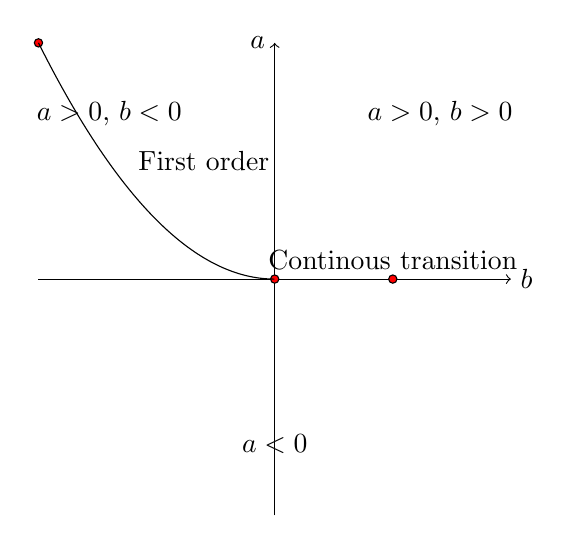
\begin{tikzpicture}[scale = 3]
        \draw[->] (-1,0) -- (1,0) node[right]{$b$}; 
        \draw[->] (0,-1) -- (0,1) node[left]{$a$}; 
        \draw[fill= red] (0,0) circle(0.5pt);
        \draw[fill= red] (.5,0) circle(0.5pt) node[above] {Continous transition};
        \draw[fill= red] (-1,1) circle(0.5pt);
        \node at (-.3, .5) {First order};
        \draw plot[domain=-1:0, samples=100] (\x, {pow(\x, 2)});
        \node at (-0.7, 0.7) {$a>0$, $b < 0$};
        \node at (0.7, 0.7) {$a>0$, $b > 0$};
        \node at (0.0, -0.7) {$a<0$};
    \end{tikzpicture}
    \caption{Phase diagram in the $a-b$ plane.}
    \label{fig: phase diagram}
\end{figure}\noindent
The region ($a>0$, $b>0$) is continuous because the derivative of $\mathcal{L}$ is the same if we go from above or below. This is in contrast to the region ($a>0$ and $b> 0$), where the derivative changes sign if we go from above or below, indicating a first order phase transition.
The region ($a<0$) is continuous because the second derivative of $\mathcal{L}$ is negative, indicating a minimum.

\newparagraph
In the below figure, the form of the Landau free energy of the system is sketched in the investigated regions, fig \ref{fig: Landau free energy}.
The point $(0,0)$ is called a tricritical point because it's the point where the phase transition changes from first order to continuous. This is because the second derivative of the Landau free energy changes sign at this point, indicating a change in the order of the phase transition.


\begin{figure}[H]
    \centering
    \begin{subfigure}[b]{0.4\textwidth}
        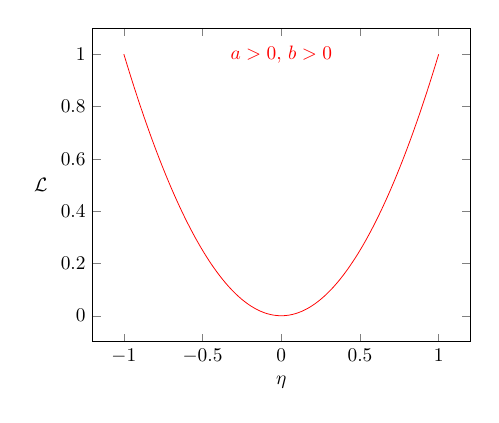
\begin{tikzpicture}[scale = 0.7]
            \begin{axis}[xlabel = {$\eta$}, ylabel = {$\mathcal{L}$}, domain=-1:1, ylabel style = {rotate = -90}]
                \addplot[samples = 100, color = red]{x^2};
                \node[color = red] at (0, 1) {$a>0$, $b > 0$};
            \end{axis}
        \end{tikzpicture}
        \caption{$\mathcal{L}$ for $a>0$, $b > 0$}
    \end{subfigure}
    \hfill
    \begin{subfigure}[b]{0.4\textwidth}
        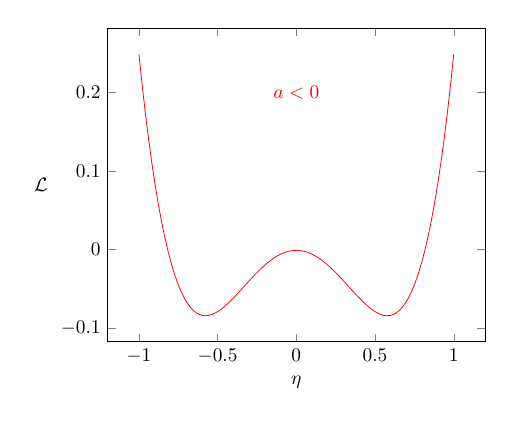
\begin{tikzpicture}[scale = 0.7]
            \begin{axis}[xlabel = {$\eta$}, ylabel = {$\mathcal{L}$}, domain=-1:1, ylabel style = {rotate = -90}]
                \addplot[samples = 100, color = red]{-0.001 + -.5 * x^2 + 0.75 * x^4};
                \node[color = red] at (0, .2) {$a<0$};
            \end{axis}
        \end{tikzpicture}
        \caption{$\mathcal{L}$ for $a<0$}
    \end{subfigure}
    \hfill
    \begin{subfigure}[b]{0.4\textwidth}
        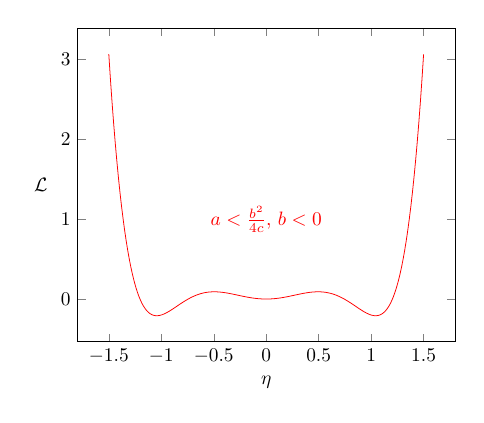
\begin{tikzpicture}[scale = 0.7]
            \begin{axis}[xlabel = {$\eta$}, ylabel = {$\mathcal{L}$}, domain=-1.5:1.5, ylabel style = {rotate = -90}]
                \addplot[samples = 200, color = red]{0.8 * x^2 -2 * x^4 + x^6};
                \node[color = red] at (0, 1) {$a<\frac{b^2}{4c}$, $b < 0$};
            \end{axis}
        \end{tikzpicture}
        \caption{$\mathcal{L}$ for $a<\frac{b^2}{4c}$, $b < 0$}
    \end{subfigure}
    \hfill
    \begin{subfigure}[b]{0.4\textwidth}
        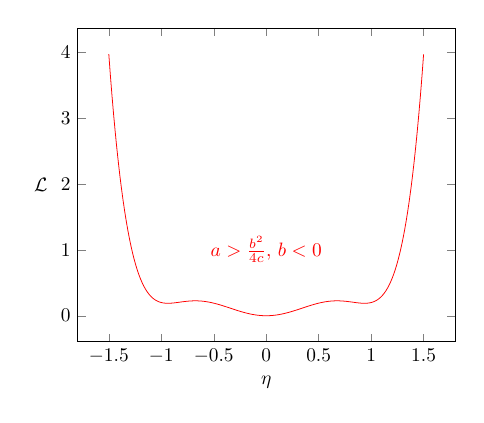
\begin{tikzpicture}[scale = 0.7]
            \begin{axis}[xlabel = {$\eta$}, ylabel = {$\mathcal{L}$}, domain=-1.5:1.5, ylabel style = {rotate = -90}]
                \addplot[samples = 200, color = red]{1.2 * x^2 -2 * x^4 + x^6};
                \node[color = red] at (0, 1) {$a>\frac{b^2}{4c}$, $b < 0$};
            \end{axis}
        \end{tikzpicture}
        \caption{$\mathcal{L}$ for $a>\frac{b^2}{4c}$, $b < 0$}
    \end{subfigure}
    \hfill
    \begin{subfigure}[b]{0.4\textwidth}
        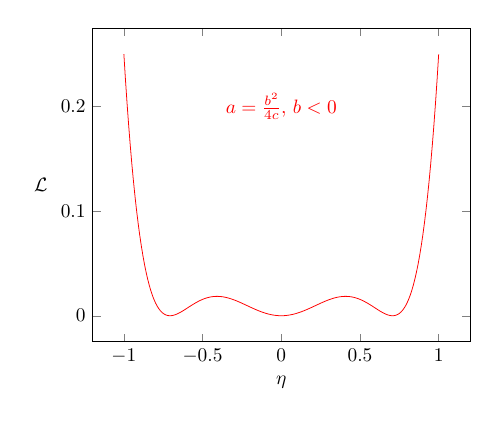
\begin{tikzpicture}[scale = 0.7]
            \begin{axis}[xlabel = {$\eta$}, ylabel = {$\mathcal{L}$}, domain=-1:1, ylabel style = {rotate = -90}]
                \addplot[samples = 200, color = red]{1/4* x^2 -1 * x^4 + x^6};
                \node[color = red] at (0, .2) {$a=\frac{b^2}{4c}$, $b < 0$};
            \end{axis}
        \end{tikzpicture}
        \caption{$\mathcal{L}$ for $a=\frac{b^2}{4c}$, $b < 0$}
    \end{subfigure}
    \caption{The form of the Landau free energy in each region.}
    \label{fig: Landau free energy}
\end{figure}


\section*{e)}
Calculate the thermodynamic critical exponents, by approaching the tricritical point along the line $b = 0$.
What do you expect $\nu$ to be?

\newparagraph
\textbf{Answer: }The Landau free energy density is given by:
\begin{align}
    \mathcal{L} &= \frac{1}{2}a\eta^2 + \frac{1}{6}c\eta^6 - h\eta\nonumber\\
    &= \frac{1}{2}\eta^2\left(a + \frac{c}{3}\eta^4\right) - h\eta,\label{eq: LFD rewrite}
\end{align}along the line $b = 0$. Differentiating this expression with respect to the order parameter $\eta$ yields:
\begin{align}
    \fpartial{\mathcal{L}}{\eta} &= a\eta + c\eta^5 - h = 0. \label{eq: LFD b = 0}
\end{align}We will approach the tricritical point along the line $b = 0$, i.e. not along the curve found in figure \ref{fig: phase diagram}, but rather the continuous phase transition. 
When $a<0$ and $h = 0$, we have the following expression:
\begin{align*}
    0 &= a\eta + c\eta^5\\
    \implies \eta &= \left(-\frac{a}{c}\right)^{1/4}.
\end{align*}Therefore, the critical exponent $\beta$ is given by: $\beta = 1/4$. If instead, the system parameters $t$ and $p$ is zero, then we obtain:
\begin{align*}
    0 &= c\eta^5 - h\\
    \implies \eta &= \left(\frac{h}{c}\right)^{1/5}.
\end{align*}Thus, the critical exponent $\delta$ is given by: $\delta = 5$.
To find the critical exponent $\nu$, we need to consider the magnetic suspectability, which is the second derivative of the Landau free energy:
\begin{align*}
    &\left(a + 5 \eta^4\right)\frac{\partial \eta}{\partial h} - 1 = 0\\
    \implies &\frac{\partial \eta}{\partial h} = \frac{1}{a + 5 \eta^4} = -\frac{1}{4a}\quad a>0.
\end{align*}This, then implies that the critical exponent $\gamma_1 = \gamma_2 = 1$. At the point $a>0$, $\eta$ is zero, and thus $\mathcal{L} = 0$. At $a<0$, the order parameter is given by $\eta = \left(\frac{-a}{4}\right)^{0.25}$.
Inserting this in eq \eqref{eq: LFD rewrite} gives us, when $h = 0$:
\begin{align*}
    \mathcal{L} &= \frac{1}{2}\eta^2 \left(a + \frac{c}{3}\eta^{4}\right)\\
    &= \frac{1}{2}\left(\frac{-a}{c}\right)^{1/2}\left(a + \frac{c}{3}\frac{-a}{c}\right)\\
    &= \frac{1}{2}\left(\frac{-a}{c}\right)^2{1/2} \left(\frac{2a}{3}\right)\\
    &= \frac{c}{3}\left(-\frac{a}{c}\right)^{3/2}\\
    &= \frac{c}{3}\left(-\frac{a_1t + a_2p}{c}\right)^{3/2}.
\end{align*}The heat capacity is proportional to the second derivative of the Landau free energy, with respect to $t$.
\begin{align*}
    C &= \fpartial{^2\mathcal{L}}{t^2},\\
    C&\sim\left(\frac{a_1t + a_2p}{c}\right)^{-\frac{1}{2}}.
\end{align*}If $a$ thus is negative, the negative heat capacity is not real, and thus $\alpha_1 = 0$, and if $a>0$ we have $\alpha_2 = \frac{1}{2}$.
The critical exponent $\nu$ is thus given by:
\begin{align*}
    &\nu = \frac{2-\alpha}{d}\\
    &= \frac{2-\frac{1}{2}}{d} = \frac{3}{d}.\\
\end{align*}We expect from lower order free energy $\frac{2}{d}$ and thus this result is plausible.


\section*{f)}
Show that for small but positive $b$, there is a crossover from the tricritical behavior which you have found to ordinary critical behavior when $b^2\sim - ac$.

\newparagraph
\textbf{Answer: }If $b>0$, then the highest order parameter can be included into the $\eta^4$ term, and thus we can write the Landau free energy as:
\begin{align*}
    \mathcal{L} &= \frac{1}{2}a\eta^2 + \frac{1}{4}b\eta^4 - h\eta.
\end{align*}This in itself is the ordinary Landau free energy, which is has known critical behavior.
Thus, each of the components are comparable,
\begin{align*}
    \frac{1}{2}\abs{a}\eta^2 &\sim \frac{1}{4}b\eta^4\implies \eta^2 \sim \frac{2\abs{a}}{b}\\
    \frac{1}{4}b\eta^4 &\sim \frac{1}{6}c\eta^6 \implies \eta^2 \sim \frac{6b}{4}.
\end{align*}Comparing the two terms we obtain:
\begin{align*}
    &\frac{2\abs{a}}{b}\sim \frac{6b}{4},\\
    \implies& b^2 \sim -ac.
\end{align*}




\end{document}
 
